\documentclass[twoside]{book}

% Packages required by doxygen
\usepackage{calc}
\usepackage{doxygen}
\usepackage{graphicx}
\usepackage[utf8]{inputenc}
\usepackage{makeidx}
\usepackage{multicol}
\usepackage{multirow}
\usepackage{fixltx2e}
\PassOptionsToPackage{warn}{textcomp}
\usepackage{textcomp}
\usepackage[nointegrals]{wasysym}
\usepackage[table]{xcolor}

% Font selection
\usepackage[T1]{fontenc}
\usepackage{mathptmx}
\usepackage[scaled=.90]{helvet}
\usepackage{courier}
\usepackage{amssymb}
\usepackage{sectsty}
\renewcommand{\familydefault}{\sfdefault}
\allsectionsfont{%
  \fontseries{bc}\selectfont%
  \color{darkgray}%
}
\renewcommand{\DoxyLabelFont}{%
  \fontseries{bc}\selectfont%
  \color{darkgray}%
}
\newcommand{\+}{\discretionary{\mbox{\scriptsize$\hookleftarrow$}}{}{}}

% Page & text layout
\usepackage{geometry}
\geometry{%
  a4paper,%
  top=2.5cm,%
  bottom=2.5cm,%
  left=2.5cm,%
  right=2.5cm%
}
\tolerance=750
\hfuzz=15pt
\hbadness=750
\setlength{\emergencystretch}{15pt}
\setlength{\parindent}{0cm}
\setlength{\parskip}{0.2cm}
\makeatletter
\renewcommand{\paragraph}{%
  \@startsection{paragraph}{4}{0ex}{-1.0ex}{1.0ex}{%
    \normalfont\normalsize\bfseries\SS@parafont%
  }%
}
\renewcommand{\subparagraph}{%
  \@startsection{subparagraph}{5}{0ex}{-1.0ex}{1.0ex}{%
    \normalfont\normalsize\bfseries\SS@subparafont%
  }%
}
\makeatother

% Headers & footers
\usepackage{fancyhdr}
\pagestyle{fancyplain}
\fancyhead[LE]{\fancyplain{}{\bfseries\thepage}}
\fancyhead[CE]{\fancyplain{}{}}
\fancyhead[RE]{\fancyplain{}{\bfseries\leftmark}}
\fancyhead[LO]{\fancyplain{}{\bfseries\rightmark}}
\fancyhead[CO]{\fancyplain{}{}}
\fancyhead[RO]{\fancyplain{}{\bfseries\thepage}}
\fancyfoot[LE]{\fancyplain{}{}}
\fancyfoot[CE]{\fancyplain{}{}}
\fancyfoot[RE]{\fancyplain{}{\bfseries\scriptsize Generated on Tue Aug 19 2014 18\+:06\+:26 for My Project by Doxygen }}
\fancyfoot[LO]{\fancyplain{}{\bfseries\scriptsize Generated on Tue Aug 19 2014 18\+:06\+:26 for My Project by Doxygen }}
\fancyfoot[CO]{\fancyplain{}{}}
\fancyfoot[RO]{\fancyplain{}{}}
\renewcommand{\footrulewidth}{0.4pt}
\renewcommand{\chaptermark}[1]{%
  \markboth{#1}{}%
}
\renewcommand{\sectionmark}[1]{%
  \markright{\thesection\ #1}%
}

% Indices & bibliography
\usepackage{natbib}
\usepackage[titles]{tocloft}
\setcounter{tocdepth}{3}
\setcounter{secnumdepth}{5}
\makeindex

% Hyperlinks (required, but should be loaded last)
\usepackage{ifpdf}
\ifpdf
  \usepackage[pdftex,pagebackref=true]{hyperref}
\else
  \usepackage[ps2pdf,pagebackref=true]{hyperref}
\fi
\hypersetup{%
  colorlinks=true,%
  linkcolor=blue,%
  citecolor=blue,%
  unicode%
}

% Custom commands
\newcommand{\clearemptydoublepage}{%
  \newpage{\pagestyle{empty}\cleardoublepage}%
}


%===== C O N T E N T S =====

\begin{document}

% Titlepage & ToC
\hypersetup{pageanchor=false,
             bookmarks=true,
             bookmarksnumbered=true,
             pdfencoding=unicode
            }
\pagenumbering{roman}
\begin{titlepage}
\vspace*{7cm}
\begin{center}%
{\Large My Project }\\
\vspace*{1cm}
{\large Generated by Doxygen 1.8.7}\\
\vspace*{0.5cm}
{\small Tue Aug 19 2014 18:06:26}\\
\end{center}
\end{titlepage}
\clearemptydoublepage
\tableofcontents
\clearemptydoublepage
\pagenumbering{arabic}
\hypersetup{pageanchor=true}

%--- Begin generated contents ---
\chapter{Namespace Index}
\section{Namespace List}
Here is a list of all documented namespaces with brief descriptions\+:\begin{DoxyCompactList}
\item\contentsline{section}{\hyperlink{namespacestd}{std} }{\pageref{namespacestd}}{}
\end{DoxyCompactList}

\chapter{Hierarchical Index}
\section{Class Hierarchy}
This inheritance list is sorted roughly, but not completely, alphabetically\+:\begin{DoxyCompactList}
\item \contentsline{section}{Hamiltonian$<$ walker $>$}{\pageref{class_hamiltonian}}{}
\begin{DoxyCompactList}
\item \contentsline{section}{Operators$<$ walker $>$}{\pageref{class_operators}}{}
\end{DoxyCompactList}
\item \contentsline{section}{std\+:\+:hash$<$ vector$<$ walker $>$ $>$}{\pageref{classstd_1_1hash_3_01vector_3_01walker_01_4_01_4}}{}
\item \contentsline{section}{Walker$<$ walker $>$}{\pageref{class_walker}}{}
\item \contentsline{section}{Wavefunction$<$ walker $>$}{\pageref{class_wavefunction}}{}
\end{DoxyCompactList}

\chapter{Class Index}
\section{Class List}
Here are the classes, structs, unions and interfaces with brief descriptions\+:\begin{DoxyCompactList}
\item\contentsline{section}{\hyperlink{class_hamiltonian}{Hamiltonian$<$ walker $>$} }{\pageref{class_hamiltonian}}{}
\item\contentsline{section}{\hyperlink{classstd_1_1hash_3_01vector_3_01walker_01_4_01_4}{std\+::hash$<$ vector$<$ walker $>$ $>$} }{\pageref{classstd_1_1hash_3_01vector_3_01walker_01_4_01_4}}{}
\item\contentsline{section}{\hyperlink{class_operators}{Operators$<$ walker $>$} }{\pageref{class_operators}}{}
\item\contentsline{section}{\hyperlink{class_walker}{Walker$<$ walker $>$} }{\pageref{class_walker}}{}
\item\contentsline{section}{\hyperlink{class_wavefunction}{Wavefunction$<$ walker $>$} }{\pageref{class_wavefunction}}{}
\end{DoxyCompactList}

\chapter{File Index}
\section{File List}
Here is a list of all documented files with brief descriptions\+:\begin{DoxyCompactList}
\item\contentsline{section}{\hyperlink{mainmp_8cpp}{mainmp.\+cpp} }{\pageref{mainmp_8cpp}}{}
\item\contentsline{section}{\hyperlink{operators_8h}{operators.\+h} }{\pageref{operators_8h}}{}
\item\contentsline{section}{\hyperlink{pairinghamiltonian_8h}{pairinghamiltonian.\+h} }{\pageref{pairinghamiltonian_8h}}{}
\item\contentsline{section}{{\bfseries randomc.\+h} }{\pageref{randomc_8h}}{}
\item\contentsline{section}{\hyperlink{walker_8h}{walker.\+h} \\*Function definitions of random number class. Uses mersenne twister algorithm }{\pageref{walker_8h}}{}
\item\contentsline{section}{\hyperlink{wavefunction_8h}{wavefunction.\+h} }{\pageref{wavefunction_8h}}{}
\end{DoxyCompactList}

\chapter{Namespace Documentation}
\hypertarget{namespacestd}{\section{std Namespace Reference}
\label{namespacestd}\index{std@{std}}
}
\subsection*{Classes}
\begin{DoxyCompactItemize}
\item 
class \hyperlink{classstd_1_1hash_3_01vector_3_01walker_01_4_01_4}{hash$<$ vector$<$ walker $>$ $>$}
\end{DoxyCompactItemize}


\subsection{Detailed Description}
This class specializes the hashing function for the vector$<$walker$>$ key and then hoists it into the std namespace. 
\begin{DoxyParams}{Parameters}
{\em rstate} & const reference to the std\+::vector being hashed into std\+::unordered\+\_\+map. \\
\hline
\end{DoxyParams}

\chapter{Class Documentation}
\hypertarget{class_hamiltonian}{\section{Hamiltonian$<$ walker $>$ Class Template Reference}
\label{class_hamiltonian}\index{Hamiltonian$<$ walker $>$@{Hamiltonian$<$ walker $>$}}
}


{\ttfamily \#include $<$pairinghamiltonian.\+h$>$}



Inheritance diagram for Hamiltonian$<$ walker $>$\+:
\nopagebreak
\begin{figure}[H]
\begin{center}
\leavevmode
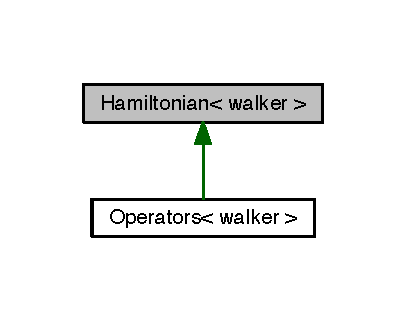
\includegraphics[width=195pt]{class_hamiltonian__inherit__graph}
\end{center}
\end{figure}
\subsection*{Public Member Functions}
\begin{DoxyCompactItemize}
\item 
\hyperlink{class_hamiltonian_a46352920e7b3584bc39c090d61d81da0}{Hamiltonian} (unsigned, unsigned, const std\+::vector$<$ double $>$ \&, const std\+::vector$<$ std\+::vector$<$ double $>$ $>$ \&)
\item 
double \hyperlink{class_hamiltonian_abd13e961c8b87b3f29a4df3781f7564e}{Hsp} (const std\+::vector$<$ walker $>$ \&) const 
\item 
double \hyperlink{class_hamiltonian_a3505c8e69ce74694dde7c4a523ca7b28}{H\+Gij} (const std\+::vector$<$ walker $>$ \&) const 
\item 
double \hyperlink{class_hamiltonian_a01979613275eed5b5c72c85a01be263a}{Diagmatrixelement} (const std\+::vector$<$ walker $>$ \&) const 
\item 
double \hyperlink{class_hamiltonian_a36a5a68b3c77370a5a4130be3393c007}{Offdiagmatrixelement} (unsigned, unsigned) const 
\item 
double \hyperlink{class_hamiltonian_ae1e4d1a832d6ce46c67a090dfe15e0b5}{Probdiagonal} (const std\+::vector$<$ walker $>$ \&) const 
\item 
double \hyperlink{class_hamiltonian_a665d48115a9a9a868328bce1537e6641}{Proboffdiagonal} (const std\+::vector$<$ walker $>$ \&) const 
\item 
double \hyperlink{class_hamiltonian_a73563fb395a29fb15daf88aaa46748e3}{shift} () const 
\end{DoxyCompactItemize}
\subsection*{Protected Attributes}
\begin{DoxyCompactItemize}
\item 
\hypertarget{class_hamiltonian_ab2981fae639bba11c2029f8f6156222f}{unsigned {\bfseries levels}}\label{class_hamiltonian_ab2981fae639bba11c2029f8f6156222f}

\item 
\hypertarget{class_hamiltonian_afe7ee42a46e4c25a3001710baadf48d4}{unsigned {\bfseries N\+P}}\label{class_hamiltonian_afe7ee42a46e4c25a3001710baadf48d4}

\item 
\hypertarget{class_hamiltonian_ad9b2f106cd03bb3607329909d65307d8}{std\+::vector$<$ double $>$ {\bfseries Esp}}\label{class_hamiltonian_ad9b2f106cd03bb3607329909d65307d8}

\item 
\hypertarget{class_hamiltonian_a12a25bd94afcb25ead9cc82864254b1c}{std\+::vector$<$ std\+::vector\\*
$<$ double $>$ $>$ {\bfseries Gij}}\label{class_hamiltonian_a12a25bd94afcb25ead9cc82864254b1c}

\end{DoxyCompactItemize}


\subsection{Detailed Description}
\subsubsection*{template$<$typename walker$>$class Hamiltonian$<$ walker $>$}

\hyperlink{class_hamiltonian}{Hamiltonian} class. walker type must be an unsigned type like uint32\+\_\+t or uint64\+\_\+t!


\begin{DoxyParams}{Parameters}
{\em N\+P} & integer value for the number of pairs. \\
\hline
{\em levels} & integer value for the number of levels. \\
\hline
{\em Esp} & std\+::vector containing the single particle energies. \\
\hline
{\em Gij} & 2-\/dimensional std\+::vector containing all the two body matrix elements Gij. \\
\hline
{\em nbits} & integer value for the number of bits in the walker data type. \\
\hline
{\em Eshift} & double value for the shift in the diagonal matrix elements.\+s\\
\hline
\end{DoxyParams}
The constructor requires as input the number of levels (levels), the number of pairs (N\+P), an std\+::vector containing the set of single particle energies $\epsilon_{k}$ (Esp), and lastly a two dimensional std\+::vector containing the set of pairing matrix elements $G_{ij}$ (Gij). 

\subsection{Constructor \& Destructor Documentation}
\hypertarget{class_hamiltonian_a46352920e7b3584bc39c090d61d81da0}{\index{Hamiltonian@{Hamiltonian}!Hamiltonian@{Hamiltonian}}
\index{Hamiltonian@{Hamiltonian}!Hamiltonian@{Hamiltonian}}
\subsubsection[{Hamiltonian}]{\setlength{\rightskip}{0pt plus 5cm}template$<$typename walker $>$ {\bf Hamiltonian}$<$ walker $>$\+::{\bf Hamiltonian} (
\begin{DoxyParamCaption}
\item[{unsigned}]{nlevels, }
\item[{unsigned}]{np, }
\item[{const std\+::vector$<$ double $>$ \&}]{r\+Esp, }
\item[{const std\+::vector$<$ std\+::vector$<$ double $>$ $>$ \&}]{r\+Gij}
\end{DoxyParamCaption}
)}}\label{class_hamiltonian_a46352920e7b3584bc39c090d61d81da0}
Constructor for the \hyperlink{class_hamiltonian}{Hamiltonian} class.


\begin{DoxyParams}{Parameters}
{\em nlevels} & integer value representing the number of levels. \\
\hline
{\em np} & integer value representing the number of pairs. \\
\hline
{\em r\+Esp} & const reference to an std\+::vector containing the single particle energies. \\
\hline
{\em r\+Gij} & const reference to a 2-\/dimensional std\+::vector containing all the two body matrix elements Gij. \\
\hline
\end{DoxyParams}


\subsection{Member Function Documentation}
\hypertarget{class_hamiltonian_a01979613275eed5b5c72c85a01be263a}{\index{Hamiltonian@{Hamiltonian}!Diagmatrixelement@{Diagmatrixelement}}
\index{Diagmatrixelement@{Diagmatrixelement}!Hamiltonian@{Hamiltonian}}
\subsubsection[{Diagmatrixelement}]{\setlength{\rightskip}{0pt plus 5cm}template$<$typename walker $>$ double {\bf Hamiltonian}$<$ walker $>$\+::Diagmatrixelement (
\begin{DoxyParamCaption}
\item[{const std\+::vector$<$ walker $>$ \&}]{rstate}
\end{DoxyParamCaption}
) const}}\label{class_hamiltonian_a01979613275eed5b5c72c85a01be263a}
This function returns a diagonal matrix element of the hamiltonian matrix i.\+e. $\langle \textbf{n}_{i} |H| \textbf{n}_{i} \rangle$. 
\begin{DoxyParams}{Parameters}
{\em rstate} & const reference to an std\+::vector representing a state in configuration space. \\
\hline
\end{DoxyParams}
\hypertarget{class_hamiltonian_a3505c8e69ce74694dde7c4a523ca7b28}{\index{Hamiltonian@{Hamiltonian}!H\+Gij@{H\+Gij}}
\index{H\+Gij@{H\+Gij}!Hamiltonian@{Hamiltonian}}
\subsubsection[{H\+Gij}]{\setlength{\rightskip}{0pt plus 5cm}template$<$typename walker $>$ double {\bf Hamiltonian}$<$ walker $>$\+::H\+Gij (
\begin{DoxyParamCaption}
\item[{const std\+::vector$<$ walker $>$ \&}]{rstate}
\end{DoxyParamCaption}
) const}}\label{class_hamiltonian_a3505c8e69ce74694dde7c4a523ca7b28}
This function returns the result of the operation of the two-\/body part of the hamiltonian on a state in configuration space. \[H_{2b}|\textbf{n} \rangle = \sum_{i,j>0}^{\omega}G_{ij}a^{\dagger}_{j}a^{\dagger}_{\tilde{j}}a_{i}a_{\tilde{i}} |\textbf{n} \rangle \]


\begin{DoxyParams}{Parameters}
{\em rstate} & const reference to an std\+::vector representing a state in configuration space. \\
\hline
\end{DoxyParams}
\hypertarget{class_hamiltonian_abd13e961c8b87b3f29a4df3781f7564e}{\index{Hamiltonian@{Hamiltonian}!Hsp@{Hsp}}
\index{Hsp@{Hsp}!Hamiltonian@{Hamiltonian}}
\subsubsection[{Hsp}]{\setlength{\rightskip}{0pt plus 5cm}template$<$typename walker $>$ double {\bf Hamiltonian}$<$ walker $>$\+::Hsp (
\begin{DoxyParamCaption}
\item[{const std\+::vector$<$ walker $>$ \&}]{rstate}
\end{DoxyParamCaption}
) const}}\label{class_hamiltonian_abd13e961c8b87b3f29a4df3781f7564e}
This function returns the result of the operation of the one-\/body part of the hamiltonian on a state in configuration space. \[H_{1b}|\textbf{n} \rangle = 2\sum_{i>0}^{\omega }\epsilon_{i}(a^{\dagger}_{i}a_{i} + a^{\dagger}_{\tilde{i}}a_{\tilde{i}}) |\textbf{n} \rangle \]


\begin{DoxyParams}{Parameters}
{\em rstate} & const reference to an std\+::vector representing a state in configuration space. \\
\hline
\end{DoxyParams}
\hypertarget{class_hamiltonian_a36a5a68b3c77370a5a4130be3393c007}{\index{Hamiltonian@{Hamiltonian}!Offdiagmatrixelement@{Offdiagmatrixelement}}
\index{Offdiagmatrixelement@{Offdiagmatrixelement}!Hamiltonian@{Hamiltonian}}
\subsubsection[{Offdiagmatrixelement}]{\setlength{\rightskip}{0pt plus 5cm}template$<$typename walker $>$ double {\bf Hamiltonian}$<$ walker $>$\+::Offdiagmatrixelement (
\begin{DoxyParamCaption}
\item[{unsigned}]{i, }
\item[{unsigned}]{j}
\end{DoxyParamCaption}
) const}}\label{class_hamiltonian_a36a5a68b3c77370a5a4130be3393c007}
This function returns an off-\/diagonal matrix element of the hamiltonian matrix i.\+e. $\langle \textbf{n}_{j} |H| \textbf{n}_{i} \rangle$. 
\begin{DoxyParams}{Parameters}
{\em rstate} & const reference to an std\+::vector representing a state in configuration space. \\
\hline
\end{DoxyParams}
\hypertarget{class_hamiltonian_ae1e4d1a832d6ce46c67a090dfe15e0b5}{\index{Hamiltonian@{Hamiltonian}!Probdiagonal@{Probdiagonal}}
\index{Probdiagonal@{Probdiagonal}!Hamiltonian@{Hamiltonian}}
\subsubsection[{Probdiagonal}]{\setlength{\rightskip}{0pt plus 5cm}template$<$typename walker $>$ double {\bf Hamiltonian}$<$ walker $>$\+::Probdiagonal (
\begin{DoxyParamCaption}
\item[{const std\+::vector$<$ walker $>$ \&}]{rstate}
\end{DoxyParamCaption}
) const}}\label{class_hamiltonian_ae1e4d1a832d6ce46c67a090dfe15e0b5}
This function returns the probability of making a diagonal transition in configuration space i.\+e. where a state transitions into the same state and no pairs are moved.

In general the set of transition probabilites are proportional to the normalized matrix elements of all states connected to the current configuration. \[\mathcal{P}_{ij} = \frac{\langle \textbf{n}_{j} |H| \textbf{n}_{i} \rangle}{d_{ij}}\] where $d_{ij} = \sum_{j} \langle \textbf{n}_{j} |H| \textbf{n}_{i} \rangle$ following the linear normalization condition.


\begin{DoxyParams}{Parameters}
{\em rstate} & const reference to an std\+::vector representing a state in configuration space. \\
\hline
\end{DoxyParams}
\hypertarget{class_hamiltonian_a665d48115a9a9a868328bce1537e6641}{\index{Hamiltonian@{Hamiltonian}!Proboffdiagonal@{Proboffdiagonal}}
\index{Proboffdiagonal@{Proboffdiagonal}!Hamiltonian@{Hamiltonian}}
\subsubsection[{Proboffdiagonal}]{\setlength{\rightskip}{0pt plus 5cm}template$<$typename walker $>$ double {\bf Hamiltonian}$<$ walker $>$\+::Proboffdiagonal (
\begin{DoxyParamCaption}
\item[{const std\+::vector$<$ walker $>$ \&}]{rstate}
\end{DoxyParamCaption}
) const}}\label{class_hamiltonian_a665d48115a9a9a868328bce1537e6641}
This function returns the probability of making a off-\/diagonal transition in configuration space i.\+e. where a state transitions into a new state and a pair is moved from an occupied level to an unoccupied level.

In general the set of transition probabilites are proportional to the normalized matrix elements of all states connected to the current configuration. \[\mathcal{P}_{ij} = \frac{\langle \textbf{n}_{j} |H| \textbf{n}_{i} \rangle}{d_{ij}}\] where $d_{ij} = \sum_{j} \langle \textbf{n}_{j} |H| \textbf{n}_{i} \rangle$ following the linear normalization condition.


\begin{DoxyParams}{Parameters}
{\em rstate} & const reference to an std\+::vector representing a state in configuration space. \\
\hline
\end{DoxyParams}
\hypertarget{class_hamiltonian_a73563fb395a29fb15daf88aaa46748e3}{\index{Hamiltonian@{Hamiltonian}!shift@{shift}}
\index{shift@{shift}!Hamiltonian@{Hamiltonian}}
\subsubsection[{shift}]{\setlength{\rightskip}{0pt plus 5cm}template$<$typename walker $>$ double {\bf Hamiltonian}$<$ walker $>$\+::shift (
\begin{DoxyParamCaption}
{}
\end{DoxyParamCaption}
) const}}\label{class_hamiltonian_a73563fb395a29fb15daf88aaa46748e3}
This function returns the diagonal shift Eshift. 

The documentation for this class was generated from the following file\+:\begin{DoxyCompactItemize}
\item 
\hyperlink{pairinghamiltonian_8h}{pairinghamiltonian.\+h}\end{DoxyCompactItemize}

\hypertarget{classstd_1_1hash_3_01vector_3_01walker_01_4_01_4}{\section{std\+:\+:hash$<$ vector$<$ walker $>$ $>$ Class Template Reference}
\label{classstd_1_1hash_3_01vector_3_01walker_01_4_01_4}\index{std\+::hash$<$ vector$<$ walker $>$ $>$@{std\+::hash$<$ vector$<$ walker $>$ $>$}}
}
\subsection*{Public Member Functions}
\begin{DoxyCompactItemize}
\item 
\hypertarget{classstd_1_1hash_3_01vector_3_01walker_01_4_01_4_ab7e3d27a8925fd17e683f2849e96ff2c}{size\+\_\+t {\bfseries operator()} (const std\+::vector$<$ walker $>$ \&rstate) const }\label{classstd_1_1hash_3_01vector_3_01walker_01_4_01_4_ab7e3d27a8925fd17e683f2849e96ff2c}

\end{DoxyCompactItemize}


The documentation for this class was generated from the following file\+:\begin{DoxyCompactItemize}
\item 
\hyperlink{wavefunction_8h}{wavefunction.\+h}\end{DoxyCompactItemize}

\hypertarget{class_operators}{\section{Operators$<$ walker $>$ Class Template Reference}
\label{class_operators}\index{Operators$<$ walker $>$@{Operators$<$ walker $>$}}
}


{\ttfamily \#include $<$operators.\+h$>$}



Inheritance diagram for Operators$<$ walker $>$\+:
\nopagebreak
\begin{figure}[H]
\begin{center}
\leavevmode
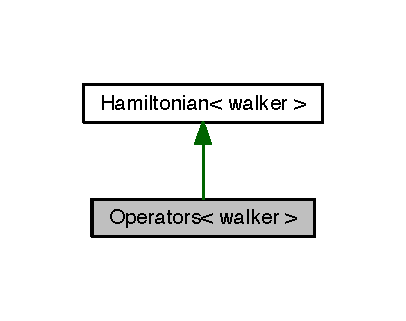
\includegraphics[width=195pt]{class_operators__inherit__graph}
\end{center}
\end{figure}


Collaboration diagram for Operators$<$ walker $>$\+:
\nopagebreak
\begin{figure}[H]
\begin{center}
\leavevmode
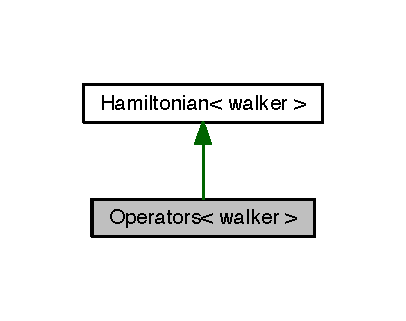
\includegraphics[width=195pt]{class_operators__coll__graph}
\end{center}
\end{figure}
\subsection*{Public Member Functions}
\begin{DoxyCompactItemize}
\item 
\hyperlink{class_operators_ae4bac9192cae36287079510f5f5dc794}{Operators} (unsigned, unsigned, const std\+::vector$<$ double $>$ \&, const std\+::vector$<$ std\+::vector$<$ double $>$ $>$ \&, const \hyperlink{class_wavefunction}{Wavefunction}$<$ walker $>$ \&)
\item 
double \hyperlink{class_operators_a047afdaf0c954f142325b8f14d9211f4}{Egs} () const 
\item 
double \hyperlink{class_operators_a6a8208aeba7b7a790d29f27574d5e435}{Expectation\+H} () const 
\item 
double \hyperlink{class_operators_ac773ffd750e58a7b7677946d2c8f7aca}{Exp\+Hsp} (typename std\+::unordered\+\_\+map$<$ std\+::vector$<$ walker $>$, double $>$\+::const\+\_\+iterator) const 
\item 
double \hyperlink{class_operators_a9b9e0389a6fc0219105959a5f9c761ad}{Exp\+H\+Gij} (typename std\+::unordered\+\_\+map$<$ std\+::vector$<$ walker $>$, double $>$\+::const\+\_\+iterator) const 
\item 
double \hyperlink{class_operators_af8b3a1ae13170fa9badcb0c35bbe25b7}{occupation\+\_\+level} (unsigned)
\item 
void \hyperlink{class_operators_a9308511b927ba7a0ca73ffc5af76ec48}{occupations} (std\+::vector$<$ double $>$ \&)
\end{DoxyCompactItemize}
\subsection*{Additional Inherited Members}


\subsection{Detailed Description}
\subsubsection*{template$<$typename walker$>$class Operators$<$ walker $>$}

Operator class. Subclasses from \hyperlink{class_hamiltonian}{Hamiltonian} class. walker type must be an unsigned type like uint32\+\_\+t or uint64\+\_\+t!


\begin{DoxyParams}{Parameters}
{\em nbits} & unsigned integer indicating the number of bits in the walker type. \\
\hline
{\em levels} & unsigned integer containing the number of levels. \\
\hline
{\em np} & unsigned integer containing the number of pairs. \\
\hline
{\em wf} & const reference to the wave function class. \\
\hline
\end{DoxyParams}


\subsection{Constructor \& Destructor Documentation}
\hypertarget{class_operators_ae4bac9192cae36287079510f5f5dc794}{\index{Operators@{Operators}!Operators@{Operators}}
\index{Operators@{Operators}!Operators@{Operators}}
\subsubsection[{Operators}]{\setlength{\rightskip}{0pt plus 5cm}template$<$typename walker $>$ {\bf Operators}$<$ walker $>$\+::{\bf Operators} (
\begin{DoxyParamCaption}
\item[{unsigned}]{nlevels, }
\item[{unsigned}]{nnp, }
\item[{const std\+::vector$<$ double $>$ \&}]{r\+Esp, }
\item[{const std\+::vector$<$ std\+::vector$<$ double $>$ $>$ \&}]{r\+Gij, }
\item[{const {\bf Wavefunction}$<$ walker $>$ \&}]{rwf}
\end{DoxyParamCaption}
)}}\label{class_operators_ae4bac9192cae36287079510f5f5dc794}
Constructor for the \hyperlink{class_operators}{Operators} class.


\begin{DoxyParams}{Parameters}
{\em nlevels} & integer value representing the number of levels. \\
\hline
{\em nnp} & integer value representing the number of pairs. \\
\hline
{\em r\+Esp} & const reference to an std\+::vector containing the single particle energies. \\
\hline
{\em r\+Gij} & const reference to a 2-\/dimensional std\+::vector containing all the two body matrix elements Gij. \\
\hline
{\em rwf} & const reference to the wave function class. \\
\hline
\end{DoxyParams}


\subsection{Member Function Documentation}
\hypertarget{class_operators_a047afdaf0c954f142325b8f14d9211f4}{\index{Operators@{Operators}!Egs@{Egs}}
\index{Egs@{Egs}!Operators@{Operators}}
\subsubsection[{Egs}]{\setlength{\rightskip}{0pt plus 5cm}template$<$typename walker $>$ double {\bf Operators}$<$ walker $>$\+::Egs (
\begin{DoxyParamCaption}
{}
\end{DoxyParamCaption}
) const}}\label{class_operators_a047afdaf0c954f142325b8f14d9211f4}
This function returns the ground state energy through the expectation value $\sum_{i} \langle \textbf{n}_{i} | H | \Psi \rangle$. This uses the non-\/standard linear normalization of the wave function. It does not require the wave function to be normalized prior to the function call. \hypertarget{class_operators_a6a8208aeba7b7a790d29f27574d5e435}{\index{Operators@{Operators}!Expectation\+H@{Expectation\+H}}
\index{Expectation\+H@{Expectation\+H}!Operators@{Operators}}
\subsubsection[{Expectation\+H}]{\setlength{\rightskip}{0pt plus 5cm}template$<$typename walker $>$ double {\bf Operators}$<$ walker $>$\+::Expectation\+H (
\begin{DoxyParamCaption}
{}
\end{DoxyParamCaption}
) const}}\label{class_operators_a6a8208aeba7b7a790d29f27574d5e435}
This function returns the ground state energy by calculating $\langle \Psi | H | \Psi \rangle$. This uses the quantum mechanical square normalization. It does not require the wave function to be normalized prior to the function call. \hypertarget{class_operators_a9b9e0389a6fc0219105959a5f9c761ad}{\index{Operators@{Operators}!Exp\+H\+Gij@{Exp\+H\+Gij}}
\index{Exp\+H\+Gij@{Exp\+H\+Gij}!Operators@{Operators}}
\subsubsection[{Exp\+H\+Gij}]{\setlength{\rightskip}{0pt plus 5cm}template$<$typename walker $>$ double {\bf Operators}$<$ walker $>$\+::Exp\+H\+Gij (
\begin{DoxyParamCaption}
\item[{typename std\+::unordered\+\_\+map$<$ std\+::vector$<$ walker $>$, double $>$\+::const\+\_\+iterator}]{it}
\end{DoxyParamCaption}
) const}}\label{class_operators_a9b9e0389a6fc0219105959a5f9c761ad}
This function returns the expectation value of the two body part of the hamiltonian in configuration space. \[ \alpha_{i}\alpha_{j} \langle \textbf{n}_{j}|H_{2b}|\textbf{n}_{i} \rangle \] \[ = \alpha_{i}\alpha_{j} \langle \textbf{n}_{j}| \sum_{i,j>0}^{\omega}G_{ij}a^{\dagger}_{j}a^{\dagger}_{\tilde{j}}a_{i}a_{\tilde{i}} |\textbf{n}_{i} \rangle \]


\begin{DoxyParams}{Parameters}
{\em it} & const iterator pointing to a state in the wave function. \\
\hline
\end{DoxyParams}
\hypertarget{class_operators_ac773ffd750e58a7b7677946d2c8f7aca}{\index{Operators@{Operators}!Exp\+Hsp@{Exp\+Hsp}}
\index{Exp\+Hsp@{Exp\+Hsp}!Operators@{Operators}}
\subsubsection[{Exp\+Hsp}]{\setlength{\rightskip}{0pt plus 5cm}template$<$typename walker $>$ double {\bf Operators}$<$ walker $>$\+::Exp\+Hsp (
\begin{DoxyParamCaption}
\item[{typename std\+::unordered\+\_\+map$<$ std\+::vector$<$ walker $>$, double $>$\+::const\+\_\+iterator}]{it}
\end{DoxyParamCaption}
) const}}\label{class_operators_ac773ffd750e58a7b7677946d2c8f7aca}
This function returns the expectation value of the one body part of the hamiltonian in configuration space. \[ \alpha_{i}^{2} \langle \textbf{n}_{i}|H_{1b}|\textbf{n}_{i} \rangle \] \[ = \alpha_{i}^{2} \langle \textbf{n}_{i}| 2\sum_{i>0}^{\omega }\epsilon_{i}(a^{\dagger}_{i}a_{i} + a^{\dagger}_{\tilde{i}}a_{\tilde{i}}) |\textbf{n}_{i} \rangle \]


\begin{DoxyParams}{Parameters}
{\em it} & const iterator pointing to a state in the wave function. \\
\hline
\end{DoxyParams}
\hypertarget{class_operators_af8b3a1ae13170fa9badcb0c35bbe25b7}{\index{Operators@{Operators}!occupation\+\_\+level@{occupation\+\_\+level}}
\index{occupation\+\_\+level@{occupation\+\_\+level}!Operators@{Operators}}
\subsubsection[{occupation\+\_\+level}]{\setlength{\rightskip}{0pt plus 5cm}template$<$typename walker $>$ double {\bf Operators}$<$ walker $>$\+::occupation\+\_\+level (
\begin{DoxyParamCaption}
\item[{unsigned}]{k}
\end{DoxyParamCaption}
)}}\label{class_operators_af8b3a1ae13170fa9badcb0c35bbe25b7}
This function computes the occupation number for the level k. The wave function should be normalized using the square norm first.


\begin{DoxyParams}{Parameters}
{\em k} & unsigned integer indicating the desired level \\
\hline
\end{DoxyParams}
\hypertarget{class_operators_a9308511b927ba7a0ca73ffc5af76ec48}{\index{Operators@{Operators}!occupations@{occupations}}
\index{occupations@{occupations}!Operators@{Operators}}
\subsubsection[{occupations}]{\setlength{\rightskip}{0pt plus 5cm}template$<$typename walker $>$ void {\bf Operators}$<$ walker $>$\+::occupations (
\begin{DoxyParamCaption}
\item[{std\+::vector$<$ double $>$ \&}]{occupationn}
\end{DoxyParamCaption}
)}}\label{class_operators_a9308511b927ba7a0ca73ffc5af76ec48}
This function calls the \hyperlink{class_operators_af8b3a1ae13170fa9badcb0c35bbe25b7}{occupation\+\_\+level()} function for each level andsaves the result into the std\+::vector occupationn.


\begin{DoxyParams}{Parameters}
{\em occupationn} & reference to an std\+::vector used to save the occupation numbers for each level. \\
\hline
\end{DoxyParams}


The documentation for this class was generated from the following file\+:\begin{DoxyCompactItemize}
\item 
\hyperlink{operators_8h}{operators.\+h}\end{DoxyCompactItemize}

\hypertarget{class_walker}{\section{Walker$<$ walker $>$ Class Template Reference}
\label{class_walker}\index{Walker$<$ walker $>$@{Walker$<$ walker $>$}}
}


{\ttfamily \#include $<$walker.\+h$>$}

\subsection*{Public Member Functions}
\begin{DoxyCompactItemize}
\item 
\hyperlink{class_walker_a5e4444d21494690947fca1eb0936c940}{Walker} (unsigned, unsigned, unsigned, double, const \hyperlink{class_wavefunction}{Wavefunction}$<$ walker $>$ \&, const \hyperlink{class_hamiltonian}{Hamiltonian}$<$ walker $>$ \&)
\item 
void \hyperlink{class_walker_a213ccb6a16ec4c211f4b15819f0ab4e4}{initialize\+\_\+walkers} (std\+::vector$<$ std\+::pair$<$ std\+::vector$<$ walker $>$, double $>$ $>$ \&)
\item 
void \hyperlink{class_walker_a1f1cefe088f5fe295e5788bb33c5b330}{random\+\_\+walk} (unsigned, std\+::vector$<$ std\+::pair$<$ std\+::vector$<$ walker $>$, double $>$ $>$ \&)
\end{DoxyCompactItemize}


\subsection{Detailed Description}
\subsubsection*{template$<$typename walker$>$class Walker$<$ walker $>$}

\hyperlink{class_walker}{Walker} class. walker type must be an unsigned type like uint32\+\_\+t or uint64\+\_\+t!


\begin{DoxyParams}{Parameters}
{\em levels} & integer value for the number of levels. \\
\hline
{\em N\+P} & integer value for the number of pairs. \\
\hline
{\em nbits} & integer value for the number of bits in the walker data type. \\
\hline
{\em wf} & const reference to a \hyperlink{class_wavefunction}{Wavefunction} class. \\
\hline
{\em H} & const reference to a \hyperlink{class_hamiltonian}{Hamiltonian} class. \\
\hline
{\em rgenerators} & an std\+::vector of mersenne generator objects. One per a thread. \\
\hline
\end{DoxyParams}


\subsection{Constructor \& Destructor Documentation}
\hypertarget{class_walker_a5e4444d21494690947fca1eb0936c940}{\index{Walker@{Walker}!Walker@{Walker}}
\index{Walker@{Walker}!Walker@{Walker}}
\subsubsection[{Walker}]{\setlength{\rightskip}{0pt plus 5cm}template$<$typename walker $>$ {\bf Walker}$<$ walker $>$\+::{\bf Walker} (
\begin{DoxyParamCaption}
\item[{unsigned}]{nthreads, }
\item[{unsigned}]{nlevels, }
\item[{unsigned}]{np, }
\item[{double}]{seed, }
\item[{const {\bf Wavefunction}$<$ walker $>$ \&}]{rwf, }
\item[{const {\bf Hamiltonian}$<$ walker $>$ \&}]{r\+H}
\end{DoxyParamCaption}
)}}\label{class_walker_a5e4444d21494690947fca1eb0936c940}
Constructor for the walker class.


\begin{DoxyParams}{Parameters}
{\em nthreads} & integer value indicating the number of threads. \\
\hline
{\em nlevels} & integer value indicating the total number of levels. \\
\hline
{\em np} & integer value indicating the total number of pairs. \\
\hline
{\em seed} & floating point initial seed value for the mersenne generator. \\
\hline
{\em rwf} & const reference to \hyperlink{class_wavefunction}{Wavefunction} class. \\
\hline
{\em r\+H} & const reference to the \hyperlink{class_hamiltonian}{Hamiltonian} class. \\
\hline
\end{DoxyParams}


\subsection{Member Function Documentation}
\hypertarget{class_walker_a213ccb6a16ec4c211f4b15819f0ab4e4}{\index{Walker@{Walker}!initialize\+\_\+walkers@{initialize\+\_\+walkers}}
\index{initialize\+\_\+walkers@{initialize\+\_\+walkers}!Walker@{Walker}}
\subsubsection[{initialize\+\_\+walkers}]{\setlength{\rightskip}{0pt plus 5cm}template$<$typename walker $>$ void {\bf Walker}$<$ walker $>$\+::initialize\+\_\+walkers (
\begin{DoxyParamCaption}
\item[{std\+::vector$<$ std\+::pair$<$ std\+::vector$<$ walker $>$, double $>$ $>$ \&}]{walkers}
\end{DoxyParamCaption}
)}}\label{class_walker_a213ccb6a16ec4c211f4b15819f0ab4e4}
This function is used to initialize the entire ensemble of walkers before the first step of the random walk. All walkers are initialized by placing all pairs into the lowest energy levels of the state.


\begin{DoxyParams}{Parameters}
{\em walkers} & reference to an std\+::vector of std\+::pairs containing all the walkers in the ensemble. \\
\hline
\end{DoxyParams}
\hypertarget{class_walker_a1f1cefe088f5fe295e5788bb33c5b330}{\index{Walker@{Walker}!random\+\_\+walk@{random\+\_\+walk}}
\index{random\+\_\+walk@{random\+\_\+walk}!Walker@{Walker}}
\subsubsection[{random\+\_\+walk}]{\setlength{\rightskip}{0pt plus 5cm}template$<$typename walker $>$ void {\bf Walker}$<$ walker $>$\+::random\+\_\+walk (
\begin{DoxyParamCaption}
\item[{unsigned}]{numsteps, }
\item[{std\+::vector$<$ std\+::pair$<$ std\+::vector$<$ walker $>$, double $>$ $>$ \&}]{walkers}
\end{DoxyParamCaption}
)}}\label{class_walker_a1f1cefe088f5fe295e5788bb33c5b330}
This function loops through the entire ensemble of walkers, from 0 to numsteps, and performs the random walk.


\begin{DoxyParams}{Parameters}
{\em numsteps} & unsigned int containing the number of single steps that occur. \\
\hline
{\em walkers} & const reference to an std\+::vector of std\+::pair containing all of the current generation of walkers. \\
\hline
\end{DoxyParams}


The documentation for this class was generated from the following file\+:\begin{DoxyCompactItemize}
\item 
\hyperlink{walker_8h}{walker.\+h}\end{DoxyCompactItemize}

\hypertarget{class_wavefunction}{\section{Wavefunction$<$ walker $>$ Class Template Reference}
\label{class_wavefunction}\index{Wavefunction$<$ walker $>$@{Wavefunction$<$ walker $>$}}
}


{\ttfamily \#include $<$wavefunction.\+h$>$}

\subsection*{Public Types}
\begin{DoxyCompactItemize}
\item 
\hypertarget{class_wavefunction_a68f7658cb4bc528aa3848329f78b54f9}{typedef std\+::unordered\+\_\+map\\*
$<$ std\+::vector$<$ walker $>$\\*
, double $>$\+::const\+\_\+iterator {\bfseries const\+\_\+iterator}}\label{class_wavefunction_a68f7658cb4bc528aa3848329f78b54f9}

\end{DoxyCompactItemize}
\subsection*{Public Member Functions}
\begin{DoxyCompactItemize}
\item 
\hypertarget{class_wavefunction_a3a714d647bd12a2517ec001ce3c03b2e}{{\bfseries Wavefunction} (unsigned, unsigned)}\label{class_wavefunction_a3a714d647bd12a2517ec001ce3c03b2e}

\item 
\hyperlink{class_wavefunction_a137b3cd275dd04a461f3f4fe11062809}{Wavefunction} (unsigned, unsigned, unsigned, unsigned)
\item 
\hyperlink{class_wavefunction_aec10cecc3b258442f3f871fff8c00ac2}{$\sim$\+Wavefunction} ()
\item 
void \hyperlink{class_wavefunction_aceb1be3ccbdd127a6d2eee3e8e9e81aa}{random\+\_\+choice} (std\+::vector$<$ std\+::pair$<$ std\+::vector$<$ walker $>$, double $>$ $>$ \&)
\item 
void \hyperlink{class_wavefunction_ae83a43a3f674f171fd469cd4850e5e7a}{weighted\+\_\+choice} (std\+::vector$<$ std\+::pair$<$ std\+::vector$<$ walker $>$, double $>$ $>$ \&)
\item 
void \hyperlink{class_wavefunction_ab9f3f8ac0b6c1343bb1c37dd0d0f2106}{insert} (const std\+::vector$<$ std\+::pair$<$ std\+::vector$<$ walker $>$, double $>$ $>$ \&)
\item 
double \hyperlink{class_wavefunction_af793b1541b937df4e668dd504fbdb18a}{configuration\+\_\+weight} (const std\+::vector$<$ walker $>$ \&) const 
\item 
void \hyperlink{class_wavefunction_afe48f8650867300927b08298736d2545}{clear} ()
\item 
void \hyperlink{class_wavefunction_aa041283ab73a60e6693446e1f45964bb}{normalise\+\_\+ln} ()
\item 
void \hyperlink{class_wavefunction_ae1c1236c133b2d375a969e765787cc7d}{normalise\+\_\+sq} ()
\item 
\hypertarget{class_wavefunction_ac83a68dc42b37228b809171b265b13d3}{const\+\_\+iterator {\bfseries begin} () const }\label{class_wavefunction_ac83a68dc42b37228b809171b265b13d3}

\item 
\hypertarget{class_wavefunction_a151f1b00cfeade0642b04e70298d069b}{const\+\_\+iterator {\bfseries end} () const }\label{class_wavefunction_a151f1b00cfeade0642b04e70298d069b}

\end{DoxyCompactItemize}


\subsection{Detailed Description}
\subsubsection*{template$<$typename walker$>$class Wavefunction$<$ walker $>$}

\hyperlink{class_wavefunction}{Wavefunction} class. walker type must be an unsigned type like uint32\+\_\+t or uint64\+\_\+t!


\begin{DoxyParams}{Parameters}
{\em N\+P} & integer value for the number of pairs. \\
\hline
{\em numlevels} & integer value for the number of levels. \\
\hline
{\em nbits} & nbits integer value for the number of bits in the walker data type. \\
\hline
{\em rgenerators} & an std\+::vector of mersenne generator objects. One per a thread. \\
\hline
{\em wave\+\_\+function} & std\+::unordered\+\_\+map container for the wave function. \\
\hline
\end{DoxyParams}


\subsection{Constructor \& Destructor Documentation}
\hypertarget{class_wavefunction_a137b3cd275dd04a461f3f4fe11062809}{\index{Wavefunction@{Wavefunction}!Wavefunction@{Wavefunction}}
\index{Wavefunction@{Wavefunction}!Wavefunction@{Wavefunction}}
\subsubsection[{Wavefunction}]{\setlength{\rightskip}{0pt plus 5cm}template$<$typename walker $>$ {\bf Wavefunction}$<$ walker $>$\+::{\bf Wavefunction} (
\begin{DoxyParamCaption}
\item[{unsigned}]{nthreads, }
\item[{unsigned}]{np, }
\item[{unsigned}]{nlevels, }
\item[{unsigned}]{seed}
\end{DoxyParamCaption}
)}}\label{class_wavefunction_a137b3cd275dd04a461f3f4fe11062809}
Constructor the \hyperlink{class_wavefunction}{Wavefunction} class.


\begin{DoxyParams}{Parameters}
{\em nthreads} & integer value representing the number of threads being used \\
\hline
{\em np} & integer value representing the number of pairs \\
\hline
{\em nlevels} & integer value representing the number of levels \\
\hline
{\em seed} & value representing the initial seed to be used to create the mersenne generator for each thread \\
\hline
\end{DoxyParams}
\hypertarget{class_wavefunction_aec10cecc3b258442f3f871fff8c00ac2}{\index{Wavefunction@{Wavefunction}!````~Wavefunction@{$\sim$\+Wavefunction}}
\index{````~Wavefunction@{$\sim$\+Wavefunction}!Wavefunction@{Wavefunction}}
\subsubsection[{$\sim$\+Wavefunction}]{\setlength{\rightskip}{0pt plus 5cm}template$<$typename walker $>$ {\bf Wavefunction}$<$ walker $>$\+::$\sim${\bf Wavefunction} (
\begin{DoxyParamCaption}
{}
\end{DoxyParamCaption}
)}}\label{class_wavefunction_aec10cecc3b258442f3f871fff8c00ac2}
Destructor the \hyperlink{class_wavefunction}{Wavefunction} class. 

\subsection{Member Function Documentation}
\hypertarget{class_wavefunction_afe48f8650867300927b08298736d2545}{\index{Wavefunction@{Wavefunction}!clear@{clear}}
\index{clear@{clear}!Wavefunction@{Wavefunction}}
\subsubsection[{clear}]{\setlength{\rightskip}{0pt plus 5cm}template$<$typename walker $>$ void {\bf Wavefunction}$<$ walker $>$\+::clear (
\begin{DoxyParamCaption}
{}
\end{DoxyParamCaption}
)}}\label{class_wavefunction_afe48f8650867300927b08298736d2545}
This function will clear the std\+::unordered\+\_\+map containing the wave function. \hypertarget{class_wavefunction_af793b1541b937df4e668dd504fbdb18a}{\index{Wavefunction@{Wavefunction}!configuration\+\_\+weight@{configuration\+\_\+weight}}
\index{configuration\+\_\+weight@{configuration\+\_\+weight}!Wavefunction@{Wavefunction}}
\subsubsection[{configuration\+\_\+weight}]{\setlength{\rightskip}{0pt plus 5cm}template$<$typename walker $>$ double {\bf Wavefunction}$<$ walker $>$\+::configuration\+\_\+weight (
\begin{DoxyParamCaption}
\item[{const std\+::vector$<$ walker $>$ \&}]{crwalker}
\end{DoxyParamCaption}
) const}}\label{class_wavefunction_af793b1541b937df4e668dd504fbdb18a}
This function returns the current weight of a configuration in the wave function. If the configuration exists then it's weight is returned otherwise 0 is returned.


\begin{DoxyParams}{Parameters}
{\em crwalker} & a const reference to an std\+::vector representing a configuration $| \textbf{n}_{i} \rangle$ \\
\hline
\end{DoxyParams}
\hypertarget{class_wavefunction_ab9f3f8ac0b6c1343bb1c37dd0d0f2106}{\index{Wavefunction@{Wavefunction}!insert@{insert}}
\index{insert@{insert}!Wavefunction@{Wavefunction}}
\subsubsection[{insert}]{\setlength{\rightskip}{0pt plus 5cm}template$<$typename walker $>$ void {\bf Wavefunction}$<$ walker $>$\+::insert (
\begin{DoxyParamCaption}
\item[{const std\+::vector$<$ std\+::pair$<$ std\+::vector$<$ walker $>$, double $>$ $>$ \&}]{walkers}
\end{DoxyParamCaption}
)}}\label{class_wavefunction_ab9f3f8ac0b6c1343bb1c37dd0d0f2106}
This function inserts an ensemble of walkers in the wave function.


\begin{DoxyParams}{Parameters}
{\em walkers} & const reference to a two dimensional std\+::vector of size equal to the number of walkers. \\
\hline
\end{DoxyParams}
\hypertarget{class_wavefunction_aa041283ab73a60e6693446e1f45964bb}{\index{Wavefunction@{Wavefunction}!normalise\+\_\+ln@{normalise\+\_\+ln}}
\index{normalise\+\_\+ln@{normalise\+\_\+ln}!Wavefunction@{Wavefunction}}
\subsubsection[{normalise\+\_\+ln}]{\setlength{\rightskip}{0pt plus 5cm}template$<$typename walker $>$ void {\bf Wavefunction}$<$ walker $>$\+::normalise\+\_\+ln (
\begin{DoxyParamCaption}
{}
\end{DoxyParamCaption}
)}}\label{class_wavefunction_aa041283ab73a60e6693446e1f45964bb}
This function normalizes the wave function following a linear normalization condition. \[Norm = \sum_{i} A_{i}\] where $A_{i}$ is the un-\/normalized amplitude of a state i in the wave function.

The result is that each amplitude $\alpha_{i}$ in the normalized wave function represents the classical probability to select the state via a random sampling. \hypertarget{class_wavefunction_ae1c1236c133b2d375a969e765787cc7d}{\index{Wavefunction@{Wavefunction}!normalise\+\_\+sq@{normalise\+\_\+sq}}
\index{normalise\+\_\+sq@{normalise\+\_\+sq}!Wavefunction@{Wavefunction}}
\subsubsection[{normalise\+\_\+sq}]{\setlength{\rightskip}{0pt plus 5cm}template$<$typename walker $>$ void {\bf Wavefunction}$<$ walker $>$\+::normalise\+\_\+sq (
\begin{DoxyParamCaption}
{}
\end{DoxyParamCaption}
)}}\label{class_wavefunction_ae1c1236c133b2d375a969e765787cc7d}
This function normalizes the wave function following a quadratic normalization condition. \[Norm = \sqrt{\sum_{i} A_{i}^{2}}\] where $A_{i}$ is the un-\/normalized amplitude of a state i in the wave function.

The result is that each amplitude $\alpha_{i}$ in the normalized wave function represents the quantum probability to select the state via a random sampling. \hypertarget{class_wavefunction_aceb1be3ccbdd127a6d2eee3e8e9e81aa}{\index{Wavefunction@{Wavefunction}!random\+\_\+choice@{random\+\_\+choice}}
\index{random\+\_\+choice@{random\+\_\+choice}!Wavefunction@{Wavefunction}}
\subsubsection[{random\+\_\+choice}]{\setlength{\rightskip}{0pt plus 5cm}template$<$typename walker $>$ void {\bf Wavefunction}$<$ walker $>$\+::random\+\_\+choice (
\begin{DoxyParamCaption}
\item[{std\+::vector$<$ std\+::pair$<$ std\+::vector$<$ walker $>$, double $>$ $>$ \&}]{walkers}
\end{DoxyParamCaption}
)}}\label{class_wavefunction_aceb1be3ccbdd127a6d2eee3e8e9e81aa}
This function randomly selects, in parallel, a new ensemble of walkers from the previous wave\+\_\+function. Each walker is represented by an std\+::pair containing an std\+::vector representing the states configuration and a double representing the amplitude. The random selection initializes the vector to a configuration existing in the wave function and sets the walkers initial amplitude to the normalized amplitude from the wave function.


\begin{DoxyParams}{Parameters}
{\em walkers} & const reference to a two dimensional std\+::vector of size equal to the number of walkers. \\
\hline
\end{DoxyParams}
\hypertarget{class_wavefunction_ae83a43a3f674f171fd469cd4850e5e7a}{\index{Wavefunction@{Wavefunction}!weighted\+\_\+choice@{weighted\+\_\+choice}}
\index{weighted\+\_\+choice@{weighted\+\_\+choice}!Wavefunction@{Wavefunction}}
\subsubsection[{weighted\+\_\+choice}]{\setlength{\rightskip}{0pt plus 5cm}template$<$typename walker $>$ void {\bf Wavefunction}$<$ walker $>$\+::weighted\+\_\+choice (
\begin{DoxyParamCaption}
\item[{std\+::vector$<$ std\+::pair$<$ std\+::vector$<$ walker $>$, double $>$ $>$ \&}]{walkers}
\end{DoxyParamCaption}
)}}\label{class_wavefunction_ae83a43a3f674f171fd469cd4850e5e7a}
This function selects via the normalized probabilities, in parallel, a new ensemble of walkers from the previous wave\+\_\+function. Each walker is represented by an std\+::pair containing an std\+::vector representing the states configuration and a double representing the amplitude. The weighted selection initializes the vector to a configuration existing in the wave function and sets the walkers initial amplitude to unity. Thus, most probable configurations are selected from the wave\+\_\+function.


\begin{DoxyParams}{Parameters}
{\em walkers} & const reference to a two dimensional std\+::vector of size equal to the number of walkers. \\
\hline
\end{DoxyParams}


The documentation for this class was generated from the following file\+:\begin{DoxyCompactItemize}
\item 
\hyperlink{wavefunction_8h}{wavefunction.\+h}\end{DoxyCompactItemize}

\chapter{File Documentation}
\hypertarget{mainmp_8cpp}{\section{mainmp.\+cpp File Reference}
\label{mainmp_8cpp}\index{mainmp.\+cpp@{mainmp.\+cpp}}
}
{\ttfamily \#include $<$fstream$>$}\\*
{\ttfamily \#include $<$iostream$>$}\\*
{\ttfamily \#include $<$cmath$>$}\\*
{\ttfamily \#include $<$ctime$>$}\\*
{\ttfamily \#include $<$utility$>$}\\*
{\ttfamily \#include $<$vector$>$}\\*
{\ttfamily \#include $<$string$>$}\\*
{\ttfamily \#include $<$omp.\+h$>$}\\*
{\ttfamily \#include \char`\"{}pairinghamiltonian.\+h\char`\"{}}\\*
{\ttfamily \#include \char`\"{}wavefunction.\+h\char`\"{}}\\*
{\ttfamily \#include \char`\"{}walker.\+h\char`\"{}}\\*
{\ttfamily \#include \char`\"{}operators.\+h\char`\"{}}\\*
Include dependency graph for mainmp.\+cpp\+:
\nopagebreak
\begin{figure}[H]
\begin{center}
\leavevmode
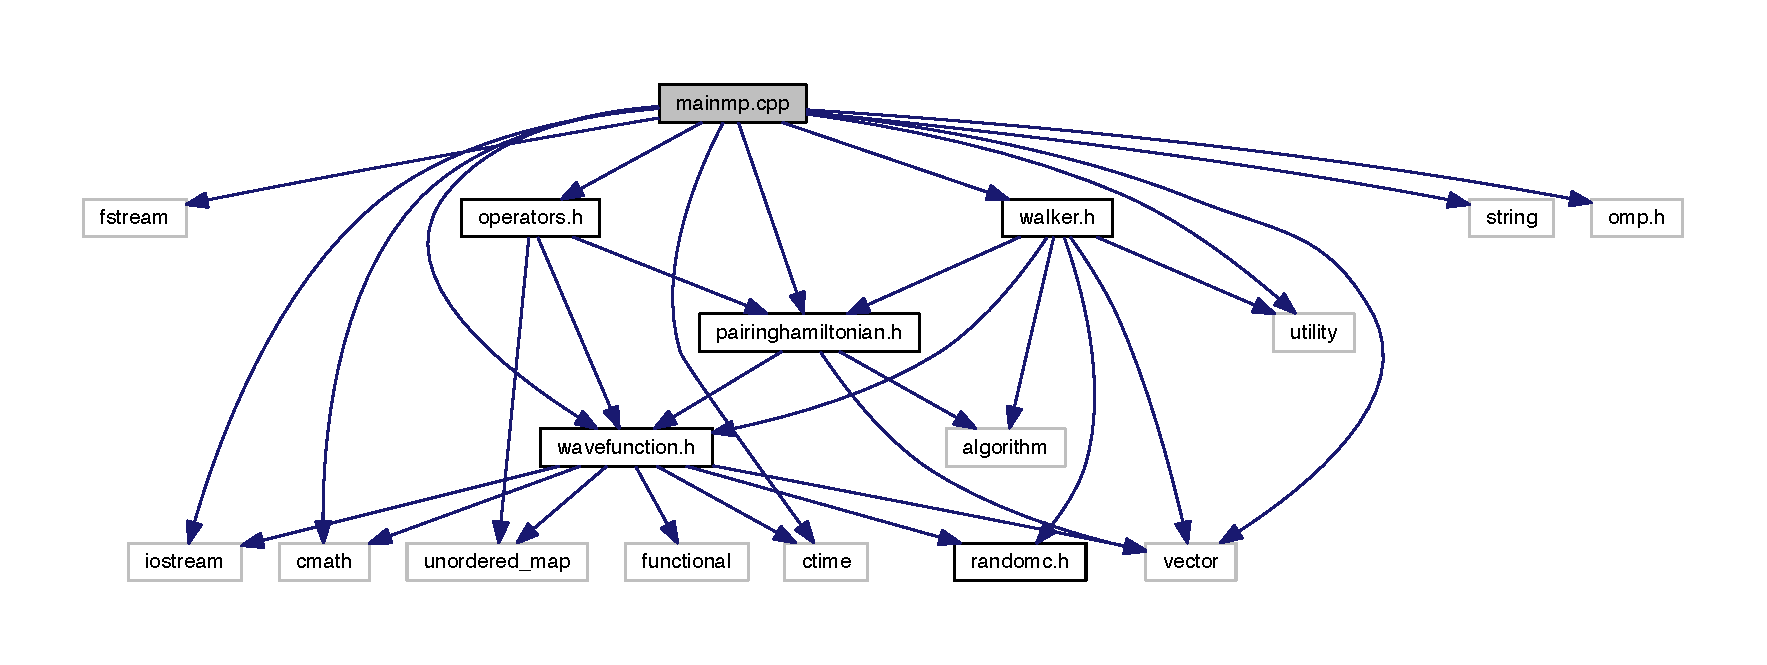
\includegraphics[width=350pt]{mainmp_8cpp__incl}
\end{center}
\end{figure}
\subsection*{Macros}
\begin{DoxyCompactItemize}
\item 
\hypertarget{mainmp_8cpp_a98f66102c54a3c53c1bf88c389f63433}{\#define {\bfseries walker\+\_\+type}~uint64\+\_\+t}\label{mainmp_8cpp_a98f66102c54a3c53c1bf88c389f63433}

\end{DoxyCompactItemize}
\subsection*{Functions}
\begin{DoxyCompactItemize}
\item 
\hypertarget{mainmp_8cpp_a72848947a8433188bbdc6ccb81ef8ef1}{double {\bfseries average} (const std\+::vector$<$ double $>$ \&)}\label{mainmp_8cpp_a72848947a8433188bbdc6ccb81ef8ef1}

\item 
\hypertarget{mainmp_8cpp_ab83397178a3535292c481582fb9db976}{double {\bfseries statistical\+\_\+error} (double, const std\+::vector$<$ double $>$ \&)}\label{mainmp_8cpp_ab83397178a3535292c481582fb9db976}

\item 
\hypertarget{mainmp_8cpp_ab3f2545adee38348b42933d73369aa17}{void {\bfseries averageoccs} (std\+::vector$<$ double $>$ \&, const std\+::vector$<$ std\+::vector$<$ double $>$ $>$ \&)}\label{mainmp_8cpp_ab3f2545adee38348b42933d73369aa17}

\item 
\hypertarget{mainmp_8cpp_a3c04138a5bfe5d72780bb7e82a18e627}{int {\bfseries main} (int argc, char $\ast$$\ast$argv)}\label{mainmp_8cpp_a3c04138a5bfe5d72780bb7e82a18e627}

\end{DoxyCompactItemize}


\subsection{Detailed Description}
This is the main file for the parallel version of the P\+M\+C software. Parallelization is implemented using Open\+M\+P. Also, c++11 support is required and the g++ -\/std=c++11 flag must be set during compilation.

It is assumed that the software will be run on a 64 bit x86 system. Thus, the unsigned data type used to represent walkers is defined as\+: \char`\"{}\#define walker\+\_\+type uint64\+\_\+t\char`\"{}. If this is not the case then this must be changed to reflect the word length of the host system. (e.\+g. uint32\+\_\+t)

An input file is required containing the parameters for the Monte Carlo evolution and the physical parameters needed to define the number of particles, levels, and various aspects of the pairing hamiltonian.

Format of input file assumes\+: 1st line\+: number of walkers (numwalkers), number of steps (numsteps), length of each step (steplength), max iterations (max\+\_\+iterations) 2nd line\+: number of pair orbitals for $\vert$n$>$ (levels), number of pairs (N\+P) 3rd line\+: s.\+p. energy of each orbital (ee) all other\+: i, j matrix indices and Gij values (Gij)

A sample input file is included labeled 2levels.\+inpt.

For the first iteration of the algorithm (equilibration step) the evolution will occur as follows. Every independent walker is initialized and then randomly walked for numsteps of length steplength. The variable steplength indicates how many random moves will take place during each numstep before the walker is saved into the wave function. After this occurs for every walker the entire wave function is then normalized and a new generation of walkers is selected via importance sampling from the previous generation. After the last numstep estimates of the ground state energy and occupation numbers are calculated.

For iterations 2 to max\+\_\+iterations, numstep is set to 1. Every independent walker is initialized via importance sampling from the result of the previous iteration. The walkers are then walked for steplength and additional estimates of the energy and occupation numbers are calculated. Every estimate is saved so that the averages and statistical errors can be computed.

The final output of the software will be the average ground state energy and it's statistical error and the occupation numbers for every level. 
\hypertarget{operators_8h}{\section{operators.\+h File Reference}
\label{operators_8h}\index{operators.\+h@{operators.\+h}}
}
{\ttfamily \#include $<$unordered\+\_\+map$>$}\\*
{\ttfamily \#include \char`\"{}pairinghamiltonian.\+h\char`\"{}}\\*
{\ttfamily \#include \char`\"{}wavefunction.\+h\char`\"{}}\\*
Include dependency graph for operators.\+h\+:
\nopagebreak
\begin{figure}[H]
\begin{center}
\leavevmode
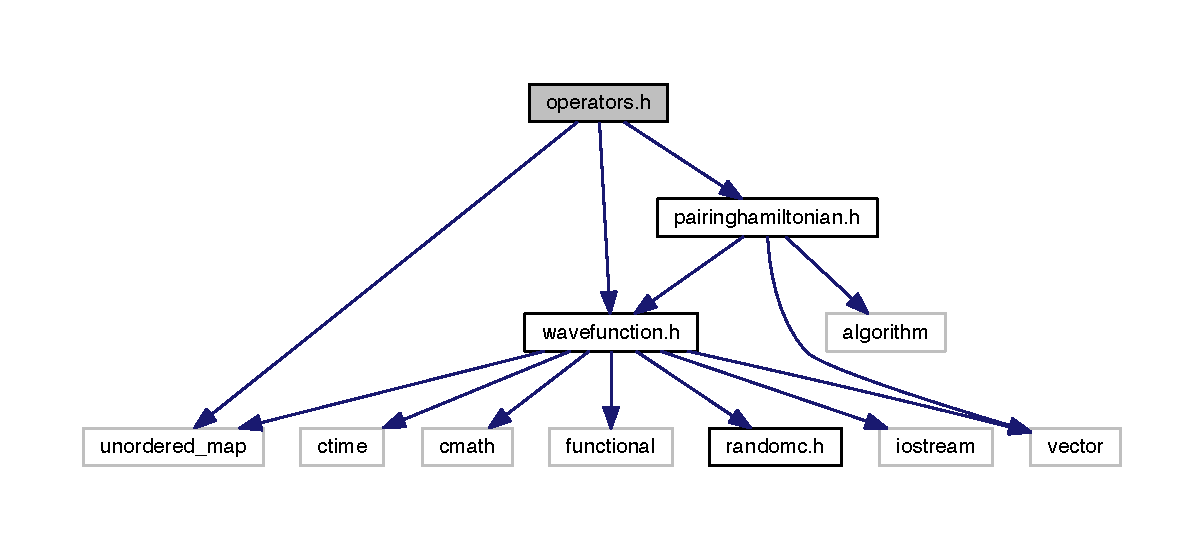
\includegraphics[width=350pt]{operators_8h__incl}
\end{center}
\end{figure}
This graph shows which files directly or indirectly include this file\+:
\nopagebreak
\begin{figure}[H]
\begin{center}
\leavevmode
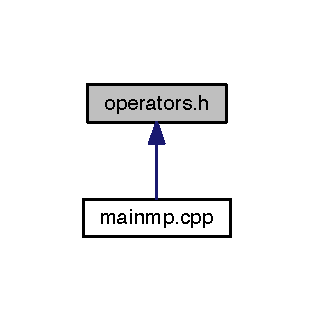
\includegraphics[width=150pt]{operators_8h__dep__incl}
\end{center}
\end{figure}
\subsection*{Classes}
\begin{DoxyCompactItemize}
\item 
class \hyperlink{class_operators}{Operators$<$ walker $>$}
\end{DoxyCompactItemize}


\subsection{Detailed Description}
This class defines the functions necessary to calculate the ground state energy expectation values, $\sum_{i} \langle \textbf{n}_{i} | H | \Psi \rangle$ and $\langle \Psi | H | \Psi \rangle$, and the occupation numbers for all levels. It inherits public and protected members from the Hamiltonian$<$walker$>$ class. This is necessary to include functions defining how the hamiltonian acts on states.

The class is templated on the unsigned integer data type chosen to represent a state in the configuration space. This can be uint32\+\_\+t, uint64\+\_\+t, or uint128\+\_\+t depending on the architecture and compiler support of the host system.

The constructor takes as input the number of levels (levels), the number of pairs (np), an std\+::vector containing the set of single particle energies $\epsilon_{k}$ (Esp), a two dimensional std\+::vector containing the set of pairing matrix elements $G_{ij}$ (Gij), and finally a const reference to the wave function (Wavefunction$<$walker$>$). 
\hypertarget{pairinghamiltonian_8h}{\section{pairinghamiltonian.\+h File Reference}
\label{pairinghamiltonian_8h}\index{pairinghamiltonian.\+h@{pairinghamiltonian.\+h}}
}
{\ttfamily \#include $<$vector$>$}\\*
{\ttfamily \#include $<$algorithm$>$}\\*
{\ttfamily \#include \char`\"{}wavefunction.\+h\char`\"{}}\\*
Include dependency graph for pairinghamiltonian.\+h\+:
\nopagebreak
\begin{figure}[H]
\begin{center}
\leavevmode
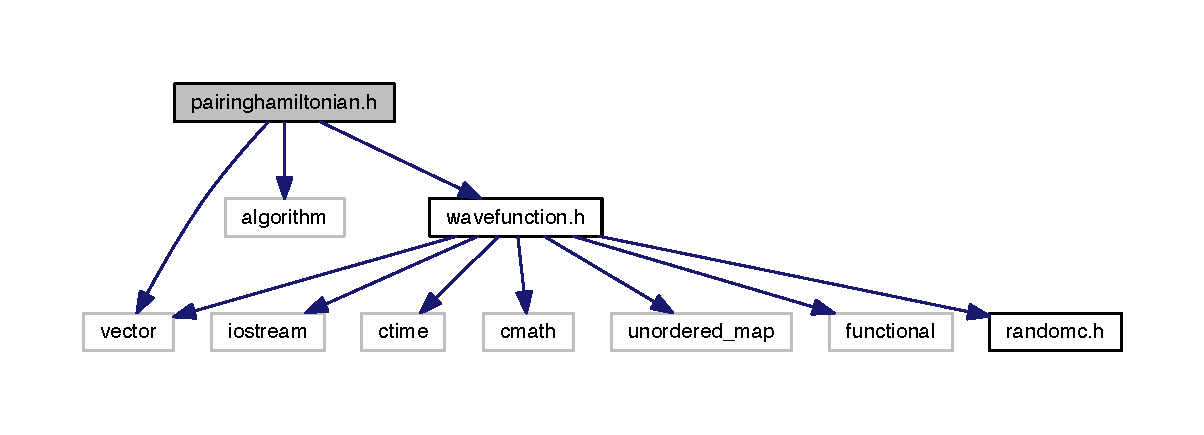
\includegraphics[width=350pt]{pairinghamiltonian_8h__incl}
\end{center}
\end{figure}
This graph shows which files directly or indirectly include this file\+:
\nopagebreak
\begin{figure}[H]
\begin{center}
\leavevmode
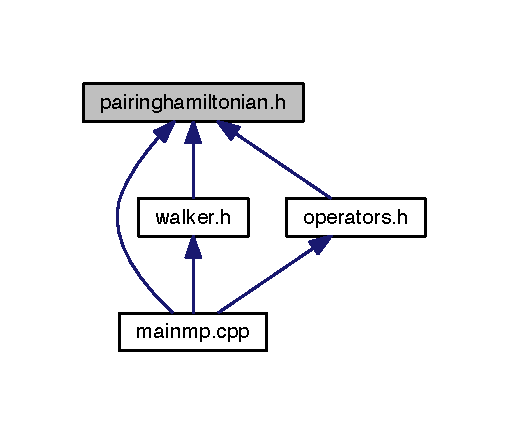
\includegraphics[width=244pt]{pairinghamiltonian_8h__dep__incl}
\end{center}
\end{figure}
\subsection*{Classes}
\begin{DoxyCompactItemize}
\item 
class \hyperlink{class_hamiltonian}{Hamiltonian$<$ walker $>$}
\end{DoxyCompactItemize}


\subsection{Detailed Description}
This class describes the pairing hamiltonian defined as \[H_{pairing} = H_{1b} + H_{2b} = 2\sum_{i>0}^{\omega }\epsilon_{i}(a^{\dagger}_{i}a_{i} + a^{\dagger}_{\tilde{i}}a_{\tilde{i}}) - \sum_{i,j>0}^{\omega}G_{ij}a^{\dagger}_{j}a^{\dagger}_{\tilde{j}}a_{i}a_{\tilde{i}}\]

The class is templated on the unsigned integer data type chosen to represent a state in the configuration space. This can be uint32\+\_\+t, uint64\+\_\+t, or uint128\+\_\+t depending on the architecture and compiler support of the host system.

The constructor requires as input the number of levels (levels), the number of pairs (N\+P), an std\+::vector containing the set of single particle energies $\epsilon_{k}$ (Esp), and lastly a two dimensional std\+::vector containing the set of pairing matrix elements $G_{ij}$ (Gij). 
\hypertarget{walker_8h}{\section{walker.\+h File Reference}
\label{walker_8h}\index{walker.\+h@{walker.\+h}}
}


Function definitions of random number class. Uses mersenne twister algorithm.  


{\ttfamily \#include $<$algorithm$>$}\\*
{\ttfamily \#include $<$vector$>$}\\*
{\ttfamily \#include $<$utility$>$}\\*
{\ttfamily \#include \char`\"{}randomc.\+h\char`\"{}}\\*
{\ttfamily \#include \char`\"{}mersenne.\+cpp\char`\"{}}\\*
{\ttfamily \#include \char`\"{}pairinghamiltonian.\+h\char`\"{}}\\*
{\ttfamily \#include \char`\"{}wavefunction.\+h\char`\"{}}\\*
Include dependency graph for walker.\+h\+:
\nopagebreak
\begin{figure}[H]
\begin{center}
\leavevmode
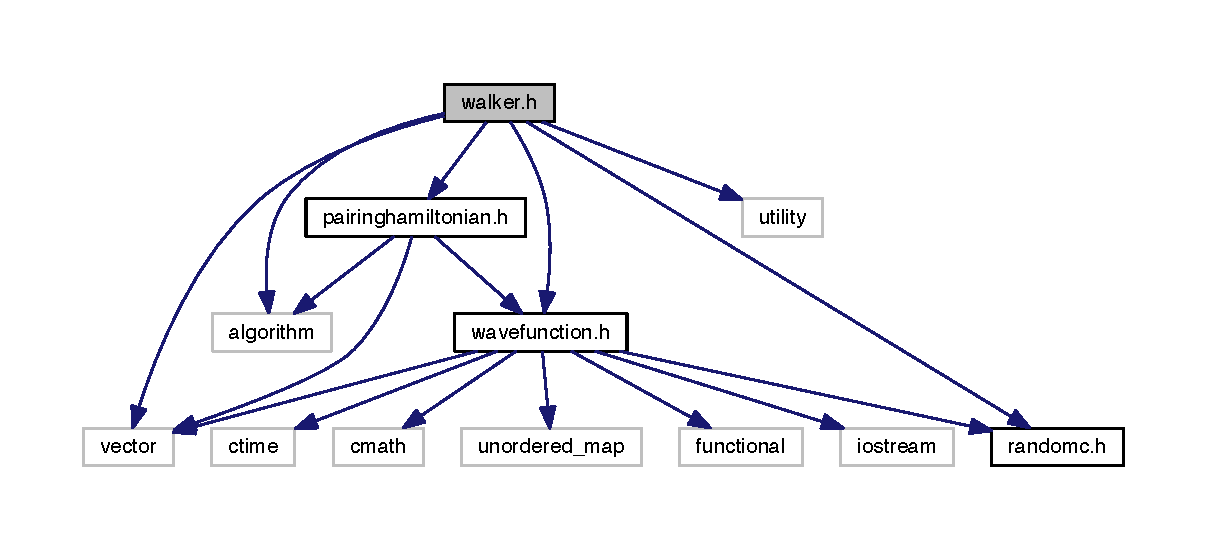
\includegraphics[width=350pt]{walker_8h__incl}
\end{center}
\end{figure}
This graph shows which files directly or indirectly include this file\+:
\nopagebreak
\begin{figure}[H]
\begin{center}
\leavevmode
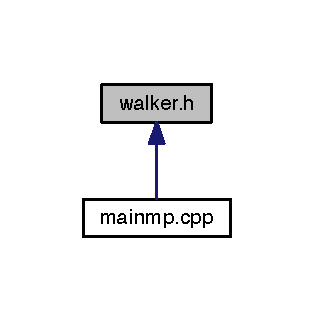
\includegraphics[width=150pt]{walker_8h__dep__incl}
\end{center}
\end{figure}
\subsection*{Classes}
\begin{DoxyCompactItemize}
\item 
class \hyperlink{class_walker}{Walker$<$ walker $>$}
\end{DoxyCompactItemize}


\subsection{Detailed Description}
Function definitions of random number class. Uses mersenne twister algorithm. 

Random number class. Uses mersenne twister algorithm.

This is the \hyperlink{class_walker}{Walker} class which handles the actual random evolution of the ensemble.

The class is templated on the unsigned integer data type chosen to represent a state in the configuration space. This can be uint32\+\_\+t, uint64\+\_\+t, or uint128\+\_\+t depending on the architecture and compiler support of the host system. 
\hypertarget{wavefunction_8h}{\section{wavefunction.\+h File Reference}
\label{wavefunction_8h}\index{wavefunction.\+h@{wavefunction.\+h}}
}
{\ttfamily \#include $<$iostream$>$}\\*
{\ttfamily \#include $<$vector$>$}\\*
{\ttfamily \#include $<$ctime$>$}\\*
{\ttfamily \#include $<$cmath$>$}\\*
{\ttfamily \#include $<$unordered\+\_\+map$>$}\\*
{\ttfamily \#include $<$functional$>$}\\*
{\ttfamily \#include \char`\"{}randomc.\+h\char`\"{}}\\*
Include dependency graph for wavefunction.\+h\+:
\nopagebreak
\begin{figure}[H]
\begin{center}
\leavevmode
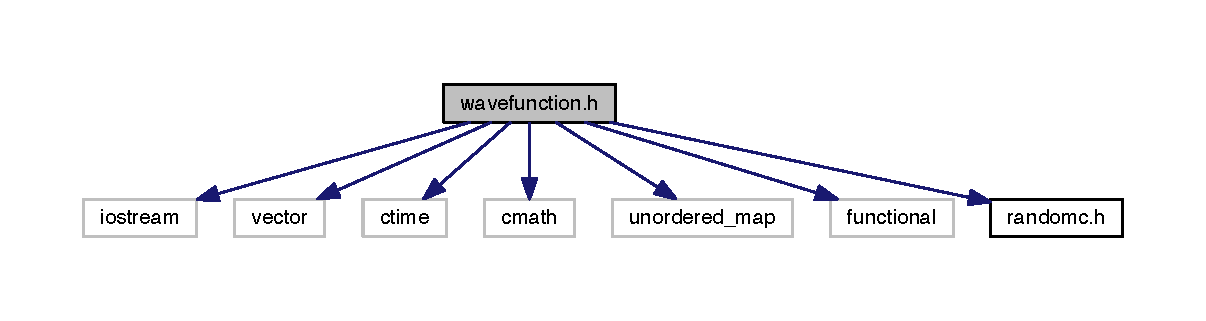
\includegraphics[width=350pt]{wavefunction_8h__incl}
\end{center}
\end{figure}
This graph shows which files directly or indirectly include this file\+:
\nopagebreak
\begin{figure}[H]
\begin{center}
\leavevmode
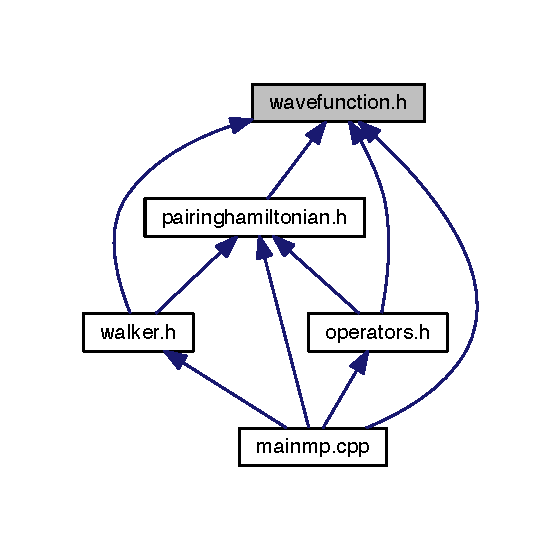
\includegraphics[width=269pt]{wavefunction_8h__dep__incl}
\end{center}
\end{figure}
\subsection*{Classes}
\begin{DoxyCompactItemize}
\item 
class \hyperlink{classstd_1_1hash_3_01vector_3_01walker_01_4_01_4}{std\+::hash$<$ vector$<$ walker $>$ $>$}
\item 
class \hyperlink{class_wavefunction}{Wavefunction$<$ walker $>$}
\end{DoxyCompactItemize}
\subsection*{Namespaces}
\begin{DoxyCompactItemize}
\item 
 \hyperlink{namespacestd}{std}
\end{DoxyCompactItemize}


\subsection{Detailed Description}
This class represents the wave function for a paired, many body wave function in configuration space \[ |\Psi \rangle = \sum _{i}^{\omega} \alpha_{i} |\textbf{n}_{i} \rangle \] where $\omega$ is the total number of different configurations, $|\textbf{n}_{i} \rangle$ is the i-\/th configuration, and $\omega$ is the amplitude of that configuration.

The underlying data structure of this class is an std\+::unordered\+\_\+map that uses contains std\+::vector$<$walker$>$/double key/value pairs.

The class is templated on the unsigned integer data type chosen to represent a state in the configuration space. This can be uint32\+\_\+t, uint64\+\_\+t, or uint128\+\_\+t depending on the architecture and compiler support of the host system.

The constructor requires as input the number of threads, the number of pairs (N\+P), the number of levels (numlevels), and the initial seed for the mersenne generator. 
%--- End generated contents ---

% Index
\newpage
\phantomsection
\addcontentsline{toc}{chapter}{Index}
\printindex

\end{document}
